\documentclass[a4paper,11pt]{article}
\usepackage{amsmath,amssymb,epsf,epsfig,times}
\usepackage[all]{xy}
\usepackage{color}
\usepackage{subfigure}
\usepackage{url,cite}
\newtheorem{theorem}{Theorem}[section]
\newtheorem{lemma}{Lemma}[section]
\def\proof{\noindent{\it Proof: }}
\def\QED{\mbox{\rule[0pt]{1.5ex}{1.5ex}}}
\def\endproof{\hspace*{\fill}~\QED\par\endtrivlist\unskip}
\newcommand{\re}{\mathbb{R}}
\def\sV{\mathcal{V}}
\def\sS{\mathcal{S}}
\def\sQ{\mathcal{Q}}

\newcommand{\mc}{\mbox{: }}

\newcommand{\normsq}[1]{\left\|#1\right\|^2}
\newcommand{\norm}[1]{\left\|#1\right\|}
%\newcommand{\sgn}[1]{\mbox{sgn}(#1)}
\newcommand{\pde}[2]{\frac{\partial #1}{\partial #2}}
\newcommand{\fundef}[3]{#1:#2\to #3}
\newcommand{\abs}[1]{\left|#1\right|}
\newcommand{\mymatrix}[2]{\left(\begin{array}{#1}#2\end{array}\right)}
\newcommand{\defeq}{\stackrel{\triangle}{=}}
\newcommand{\paren}[1]{\left(#1\right)}
%\theoremstyle{plain} \newtheorem{theorem}{Theorem}
%\theoremstyle{plain} \newtheorem{algorithm}{Algorithm}
\newtheorem{axiom}[theorem]{Axiom}
\newtheorem{definition}[theorem]{Definition}
\newtheorem{assumption}[theorem]{Assumption}
\newtheorem{example}[theorem]{Example}
%\theoremstyle{plain}\newtheorem{lemma}{Lemma}
%\newtheorem{proposition}[theorem]{Proposition}
\newtheorem{remark}[theorem]{Remark}
\newtheorem{corollary}[theorem]{Corollary}

\newcommand{\Acal}{\mathcal{A}}
\newcommand{\Bcal}{\mathcal{B}}
\newcommand{\Ccal}{\mathcal{C}}
\newcommand{\Dcal}{\mathcal{D}}
\newcommand{\Ecal}{\mathcal{E}}
\newcommand{\Fcal}{\mathcal{F}}
\newcommand{\Gcal}{\mathcal{G}}
\newcommand{\Hcal}{\mathcal{H}}
\newcommand{\Ical}{\mathcal{I}}
\newcommand{\Jcal}{\mathcal{J}}
\newcommand{\Kcal}{\mathcal{K}}
\newcommand{\Lcal}{\mathcal{L}}
\newcommand{\Mcal}{\mathcal{M}}
\newcommand{\Ncal}{\mathcal{N}}
\newcommand{\Ocal}{\mathcal{O}}
\newcommand{\Pcal}{\mathcal{P}}
\newcommand{\Qcal}{\mathcal{Q}}
\newcommand{\Rcal}{\mathcal{R}}
\newcommand{\Scal}{\mathcal{S}}
\newcommand{\Tcal}{\mathcal{T}}
\newcommand{\Ucal}{\mathcal{U}}
\newcommand{\Vcal}{\mathcal{V}}
\newcommand{\Wcal}{\mathcal{W}}
\newcommand{\Xcal}{\mathcal{X}}
\newcommand{\Ycal}{\mathcal{Y}}
\newcommand{\Zcal}{\mathcal{Z}}


\def\omegavec{\boldsymbol{\omega}}
\newcommand{\alphabf}{\boldsymbol{\alpha}}
\newcommand{\omegabf}{\boldsymbol{\omega}}
\def\omegavec{\boldsymbol{\omega}}
\newcommand{\taubf}{\boldsymbol{\tau}}
\newcommand{\qbf}{\mathbf{q}}
\newcommand{\ybf}{\mathbf{y}}
\newcommand{\pbf}{\mathbf{p}}
\newcommand{\rbf}{\mathbf{r}}
\newcommand{\ebf}{\mathbf{e}}
\newcommand{\onebf}{\mathbf{1}}
\newcommand{\zerobf}{\mathbf{0}}
\newcommand{\abf}{\mathbf{a}}
\newcommand{\ibf}{\mathbf{i}}
\newcommand{\jbf}{\mathbf{j}}
\newcommand{\kbf}{\mathbf{k}}
\newcommand{\vbf}{\mathbf{v}}
\newcommand{\wbf}{\mathbf{\omega}}
\newcommand{\fbf}{\mathbf{f}}
\newcommand{\zbf}{\mathbf{z}}
\newcommand{\xbf}{\mathbf{x}}
\newcommand{\dbf}{\mathbf{d}}
\newcommand{\Rbf}{\mathbf{R}}
\newcommand{\Tbf}{\mathbf{T}}

\newcommand{\Cbf}{\mathbf{C}}
\newcommand{\Ibf}{\mathbf{I}}
\newcommand{\Pbf}{\mathbf{P}}
\newcommand{\Qbf}{\mathbf{Q}}
\newcommand{\Vbf}{\mathbf{V}}
\newcommand{\Jbf}{\mathbf{J}}
\newcommand{\Xbf}{\mathbf{X}}
\newcommand{\Abf}{\mathbf{A}}
\newcommand{\Kbf}{\mathbf{K}}
\newcommand{\Gammabf}{\boldsymbol{\Gamma}}
\newcommand{\nubf}{\boldsymbol{\nu}}
\newcommand{\xibf}{\boldsymbol{\xi}}
\newcommand{\Xibf}{\boldsymbol{\Xi}}
\newcommand{\Omegabf}{\boldsymbol{\Omega}}


\newcommand{\ubf}{\mathbf{u}}

\newcommand{\lth}{\ell{\text{th}}}
\newcommand{\ith}{i{\text{th}}}
\newcommand{\jth}{j{\text{th}}}
\newcommand{\kth}{k{\text{th}}}
\newcommand{\ip}[2]{\left<#1,~#2\right>}

\newcommand{\OMIT}[1]{}

%%%%%%%%%%%%%%%%%%%%%%%%%%%%%%%%%%%%%%%%%%%%%%%%%%%%%%%%%
%                End Macros
%%%%%%%%%%%%%%%%%%%%%%%%%%%%%%%%%%%%%%%%%%%%%%%%%%%%%%%%%
\title{Homework}
%
%\author{Jie Mei, Wei Ren and Guangfu Ma % <-this % stops a space
%\thanks{Jie Mei and Wei Ren are with the Department of Electrical
%and Computer Engineering,
%       Utah State University, Logan, UT 84322, USA.
%       {Email: wei.ren@usu.edu}.}
%       \thanks{Guangfu Ma is with the Department of Control Science and Engineering,
%       Harbin Institute of Technology, Heilongjiang 150001, P. R. China.}
%      % \thanks{This work was supported by a National Science
%%Foundation CAREER Award (ECCS--0748287).}}
%\usepackage{amsmath}
%\newtheorem{theorem}{Theorem}[section]
%\newtheorem{lemma}{Lemma}[section]
%\newtheorem{remark}{Remark}[section]
%\newtheorem{definition}{Definition}[section]
%\newcommand{\defeq}{\stackrel{\triangle}{=}}
% correct bad hyphenation here
\hyphenation{op-tical net-works semi-conduc-tor}
%\markboth{Submitted to IEEE Transactions on Control Systems
%Technology as a Brief Paper}
%         {Submitted to IEEE Transactions on Control Systems
%Technology as a Brief Paper}

\begin{document}
\maketitle



%This paper concerns the formation problem of multi-agent systems with relative measurements. A unified formulation is proposed using a transformation matrix set of local frames.
%This paper is well written, technical sound, and contains some interesting results. Below are some comments.
%
%1. To my understanding, the transformation used in this paper is linear with respect to the relative position measurements in the global coordinate. However, some measurements, for
%example, the relative distance and the relative angles, are not linear with respect to the relative position measurements. Furthermore, the dimensions of available relative
%measurement may be different from the relative position measurements. Can the proposed formulation be used for the situations above?
%
%2. It seems that the dynamics of the agents is not discussed in the paper, where a simple integrator is considered. How about the cases of general agent dynamics? For examples,
%the double and high-order integrators, and even nonlinear agent dynamics.
%
%3. A gradient-flow approach is employed to derive the control algorithm, which, in my opinion, requires a symmetric pattern of the network topology. Therefore, the
%proposed formulation only works for undirected graphs. How about the general case of a directed graph.
%
%4. The clique-rigidity is defined in a mathematical way. Some physical explanation is welcome.
%
%5. Typos: Equation in Example 6: 1_3 and 1_5 should be 1_3^T and 1_5^T.




\begin{enumerate}


   \item Consider the system defined by the following equations:
 \begin{align*}
 \dot x_1=&~\frac{2}{3}x_2\\
 \dot x_2=&~-x_1+x_2(1-3x_1^2-2x_2^2)
 \end{align*}
\begin{itemize}
  \item[(a)] Show that the points defined by (i) $x=(0,0)$ and (ii) $1-(3x_1^2+2x_2^2)=0$ are invariant sets.
  \item[(b)] Study the stability of the origin and the invariant set $1-(3x_1^2+2x_2^2)=0$, respectively, using LaSalle's Invariant Theorem.
\end{itemize}

 \item It is known that a given dynamical system with the state $x=(x_1,x_2)$ has an equilibrium point at the origin. For this system, a function $V(\cdot)$ have been proposed, and its derivative $\dot V(\cdot)$
 has been computed. Assuming that $V(\cdot)$ and $\dot V(\cdot)$ are given below you are asked to classify the origin, in each case, as (a) stable, (b) locally uniformly asymptotically stable, and/or (c) globally uniformly asymptotically stable. Explain you answer in each case.

 \begin{itemize}
 \item[(i)] $V(x,t)=x_1^2+x_2^2$, $\dot V(x,t)=-x_1^2$.
\item[(ii)] $V(x,t)=x_1^2+x_2^2$, $\dot V(x,t)=-(x_1^2+x_2^2)e^{-t}$.
\item[(iii)] $V(x,t)=x_1^2+x_2^2$, $\dot V(x,t)=-(x_1^2+x_2^2)e^{t}$.
\item[(iv)] $V(x,t)=(x_1^2+x_2^2)e^t$, $\dot V(x,t)=-(x_1^2+x_2^2)(1+\sin^2t)$.
\item[(v)] $V(x,t)=(x_1^2+x_2^2)e^{-t}$, $\dot V(x,t)=-(x_1^2+x_2^2)$.
\item[(vi)] $V(x,t)=(x_1^2+x_2^2)(1+e^{-t})$, $\dot V(x,t)=-x_1^2e^{-t}$.
\item[(vii)] $V(x,t)=(x_1^2+x_2^2)(1+\cos^2t)$, $\dot V(x,t)=-(x_1^2+x_2^2)e^{-t}$.
\item[(viii)] $V(x,t)=(x_1^2+x_2^2)(1+\cos^2t)$, $\dot V(x,t)=-(x_1^2+x_2^2)(1+e^{-t})$.
 \end{itemize}


  \item A pendulum with time-varying friction is represented by
 \begin{align}
 \dot x_1=&~x_2,\\
 \dot x_2=&~-\sin x_1-g(t)x_2.
 \end{align}
 Suppose that $g(t)$ is continuously differentiable and satisfies
 \begin{align*}
 0<a<\alpha\leq g(t)\leq \beta<\infty ~~~~~\mbox{and}~~~~~~\dot g(t)\leq \gamma<2
 \end{align*}
 for all $t\geq 0$. Consider the Lyapunov function candidate
 \begin{align}
 V(t,x)=\frac{1}{2}(a\sin x_1+x_2)^2+[1+ag(t)-a^2](1-\cos x_1)
 \end{align}
  \begin{itemize}
 \item[(a)] Show that $V(t,x)$ is positive definite and decrescent.

   \item[(b)]
   Show that
   \begin{align}
   \dot V\leq-(\alpha-a)x_2^2-a(2-\gamma)(1-\cos x_1)+O(\|x\|^3),
   \end{align}
where $O(\|x\|^3)$ is a term bounded by $k\|x\|^3$ in some neighborhood of the origin.

   \item[(c)] Show that the origin is uniformly asymptotically stable.
 \end{itemize}


  \item We denote by $|x|$ the absolute value of $x$ if $x$ is scalar and the euclidean norm of $x$ is $x$ is a
  vector. For functions of time, the $L_2$ norm is given by
  \begin{align}
  \|x\|_p=\left(\int_0^{\infty}|x(\tau)|^p\mbox{d}\tau\right)^{\frac{1}{p}},
  \end{align}
 for $p\in[1,\infty]$, while
  \begin{align}
  \|x\|_{\infty}=\sup_{t\geq 0} |x(t)|.
  \end{align}
 We say that $x\in\mathbb{L}_p$ when $\|x\|_p<\infty$.


\begin{itemize}
  \item Write down the Barbalat's lemma, the Lyapunov-like lemma, and the Lashalle-Yoshizawa theorem.
  \item Use Barbalat's lemma to prove the Lyapunov-like lemma, Lashalle-Yoshizawa theorem, and the following corollary.

 \begin{corollary}
 If $x\in \mathbb{L}_2\bigcap\mathbb{L}_{\infty}$ and $\dot x\in \mathbb{L}_{\infty}$, then $\lim_{t\to\infty}x(t)=0$.
 \end{corollary}
\end{itemize}

%{\it Note: For the proof of Lashalle-Yoshizawa theorem, one useful fact is that a continuous function on a closed compact set is always uniformly continuous.}


\item Consider the following multi-dimensional system
\begin{align*}
\dot x = A x +B(u+\Theta^T\Phi(x))
\end{align*}
where $x\in\re^n$ is the state, $A\in\re^{n\times n}$, $B\in\re^{n\times m}$ are known matrices, $u\in\re^m$ is the control input, $\Phi(x)\in\re^{k}$ is a bounded function, and $\Theta\in \re^{k\times m}$ is an unknown constant matrix. Assume that $(A,B)$ is contrllable.
\begin{itemize}
  \item Design an adaptive control law to stabilize the system.
  \item Design an adaptive control law with adaptive $\sigma-$ modification to stabilize the system.
\end{itemize}

\item The dynamic equations of a robot manipulator in closed form are always written in the form of Euler-Lagrange equation. A dynamical system with $p$ degrees of freedom can be described
   by the EL equations as
   \begin{equation}\label{system}
    M(q)\ddot q+C(q,\dot q)\dot
    q+g(q)=\tau,
    \end{equation}
where $q\in \mathbb{R}^p$ is the vector of generalized
coordinates, $M_i(q_i)\in\mathbb{R}^{p\times p}$ is the symmetric
positive definite inertia matrix, $C(q,\dot q)\dot q\in
\mathbb{R}^p$ is the vector of Coriolis and centrifugal forces,
$g(q)$ is the vector of gravitational force, and $\tau_i\in
\mathbb{R}^p$ is the vector of control force. And it has the following properties:

\vspace{0.3cm}

{\bf Properties:}\\
  1) $M_q$ is positive definite and $k_{\underline{m}}x^Tx\leq x^TMx\leq k_{\overline{m}}x^Tx$; $\|C(x,y)z\|\leq k_C\|y\|\|z\|$. \\
  2) $\dot M(q)-2C(q,\dot q)$ is skew symmetric. \\
 3) $M(q)x+C(q,\dot q)y+g(q)=Y(q,\dot q,y,x)\Theta$,
where $Y(q,\dot q,y,x)$ is the regressor and $\Theta$ is an unknown but
constant vector.

The following shows a two-link robotic manipulator and its corresponding dynamics.
   \begin{figure}[bh]
      \centering
      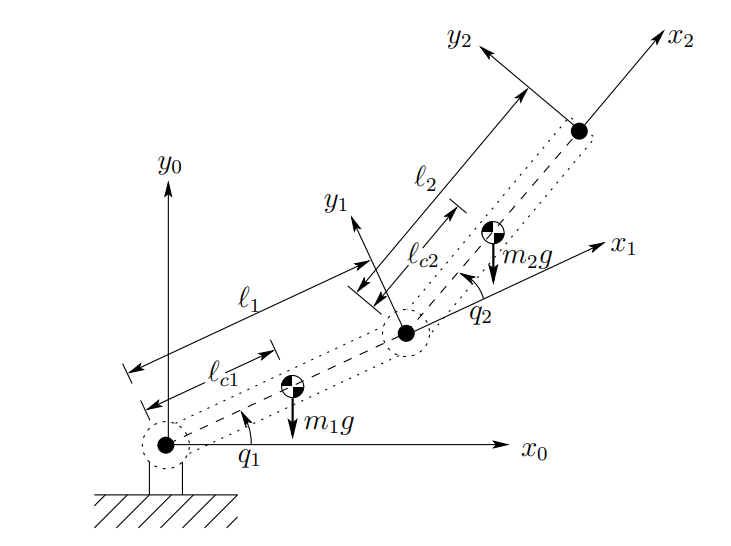
\includegraphics[width=2.5in]{figures/2linkarm}
   \end{figure}

\begin{equation}\nonumber
   M(q)=\left[
\begin{array}{cc}
               \Theta_{1}+2\Theta_{2}\cos(q_{2}) &  \Theta_{3}+\Theta_{2}\cos(q_{2})\\
               \Theta_{3}+\Theta_{2}\cos(q_{2})  &  \Theta_{3}
             \end{array}
              \right],
\end{equation}
\begin{equation}\nonumber
    C(q, \dot q)=\left[
\begin{array}{cc}
               -\Theta_{2}\sin(q_{2})\dot q_{2} &  -\Theta_{2}\sin(q_{2})(\dot q_{2}+\dot q_{1})\\
               \Theta_{2}\sin(q_{2})\dot q_{1}  &  0
             \end{array}
              \right],
\end{equation}
\begin{equation}\nonumber
    g(q)=\left[
\begin{array}{c}
               \Theta_{4}g\cos(q_{1})+\Theta_{5}g\cos(q_{1}+q_{2})\\
               \Theta_{5}g\cos(q_{1}+q_{2})
             \end{array}
              \right],
\end{equation}

\begin{align*}
\Theta=&[\Theta_{1}, \Theta_{2}, \Theta_{3},\Theta_{4},
\Theta_{5}] \\
=&[m_1l_{c1}^2\!\!+\!\!m_2(l_1^2\!\!+\!\!l_{c2}^2)\!\!+\!\!J_1\!\!+\!\!J_2, m_2l_1l_{c2},
m_2l_{c2}^2\!\!+\!\!J_2, m_1l_{c1}\!\!+\!\!m_2l_1, m_2l_{c2}],
\end{align*}

\begin{align*}
Y\!\!=\!\!\!\left[\begin{array}{ccccc}
                \!\!x_{1} & \!\!\!\cos (q_{2})\!(2x_{1}\!+\!x_{2})\!\!-\!\!\sin(q_{2})[y_{1}\!\dot q_{2}\!+\!y_{2}\!(\dot q_{1}\!+\!\dot q_{2})]&\!\!x_{2}&\!\!\!g\!\cos(q_{1})&\!\!\!g\!\cos(q_{1}\!+\!q_{2}) \\
                \!\! 0 & \!\!\cos (q_{2})x_{1}+\sin(q_{2})y_{1}\dot q_{1}& x_{1}\!\!+\!x_{2}&0&\!\!\!g\!\cos(q_{1}\!+\!q_{2})
             \end{array}
              \right].\nonumber
\end{align*}


The masses of links 1 and 2 of the
revolute joint arm are, respectively, $m_{1}=1~\mbox{kg}$
and $m_{2}=1.5~\mbox{kg}$, the lengths of links 1 and 2 are, respectively,
$l_{1}=0.2~\mbox{m}$ and $l_{2}=0.3~\mbox{m}$, the
distances from the previous joint to the center of mass of links 1
and 2 are, respectively,
$l_{c1}=0.1~\mbox{m}$ and $l_{c2}=0.15~\mbox{m}$. The moments of inertia of links 1 and 2 are,
respectively, $J_1=0.013\mbox{kg m}^2$ and $J_2=0.045~\mbox{kg m}^2$. Use the following control law
\begin{align}
\tau=-K_1(q-q_d)-K_2(\dot q - \dot q_d) + M(q)\ddot q_d +C(q,\dot q)\dot q_d+g(q)
\end{align}
where $K_1$ and $K_2$ are positive definite matrices, $q_d$ is the desired tracking trajectory. Perform simulation in the following cases and draw the errors $q-q_d$ and $\dot q-\dot q_d$.
\begin{itemize}
  \item[(a)] $q_d=[0.3, 0.1], \dot q_d=[0, 0], q(0)=\dot q(0) =[0, 0]$;
  \item[(b)] $q_d=[0.3+0.02\sin t, 0.1+0.01\cos t], \dot q_d =[0.02\cos t, -0.01\sin t], q(0)=\dot q(0) =[0,0]$;
\end{itemize}
\end{enumerate}

%\bibliographystyle{IEEEtran}
%\bibliography{../../refs}
\end{document}
